% This is a (brief) model paper using the achemso class
% The document class accepts keyval options, which should include
% the target journal and optionally the manuscript type.

\documentclass[journal=langd5, manuscript=article, layout=onecolumn]{achemso}

% Place any additional packages needed here.  Only include packages
% which are essential, to avoid problems later. Do NOT use any
% packages which require e-TeX (for example etoolbox): the e-TeX
% extensions are not currently available on the ACS conversion
% servers.

\usepackage[version=3]{mhchem} % Formula subscripts using \ce{}
\usepackage[T1]{fontenc}       % Use modern font encodings
\usepackage{amsmath, amssymb, amsfonts, gensymb}
\usepackage{graphicx}

% If issues arise when submitting your manuscript, you may want to
% un-comment the next line.  This provides information on the
% version of every file you have used.
%\listfiles

% Place any additional macros here.  Please use \newcommand* where
% possible, and avoid layout-changing macros (which are not used
% when typesetting).


\graphicspath{ {Figures/} }
\newcommand{\tdc}[3][]{\frac{\mathrm{d}^{#1}#2}{\mathrm{d}#3^{#1}}} % total differential change.
\newcommand{\pdc}[3][]{\frac{\partial^{#1} #2}{\partial #3^{#1}}} % partial differential change.
\newcommand{\td}[1]{\mathrm{d}#1}
\newcommand{\pd}[1]{\partial#1}

% Meta-data block
% ---------------
% Each author should be given as a separate \author command.
%
% Corresponding authors should have an e-mail given after the author
% name as an \email command. Phone and fax numbers can be given
% using \phone and \fax, respectively; this information is optional.
% The affiliation of authors is given after the authors; each
% \affiliation command applies to all preceding authors not already
% assigned an affiliation.
%
% The affiliation takes an option argument for the short name.  This
% will typically be something like "University of Somewhere".
% The \altaffiliation macro should be used for new address, etc.
% On the other hand, \alsoaffiliation is used on a per author basis
% when authors are associated with multiple institutions.

\author{V. S. Akella}
\affiliation{Collective Interactions Unit, OIST Graduate University, Okinawa, Japan 904-0495}
\author{D. K. Singh}
\affiliation{Collective Interactions Unit, OIST Graduate University, Okinawa, Japan 904-0495}
\author{S. Mandre}
\affiliation{School of Engineering, Brown University, 182 Hope Street, Providence, RI 02906, USA}
\author{M. M. Bandi}
\affiliation{Collective Interactions Unit, OIST Graduate University, Okinawa, Japan 904-0495}
\email{bandi@oist.jp}

% The document title should be given as usual. Some journals require
% a running title from the author: this should be supplied as an
% optional argument to \title.

\title[]{Dynamics of a self-propelled Camphoric Acid boat at the air-water interface} 

% Some journals require a list of abbreviations or keywords to be
% supplied. These should be set up here, and will be printed after
% the title and author information, if needed.

\abbreviations{IR,NMR,UV}
\keywords{Marangoni flow, Self-propulsion}

% The manuscript does not need to include \maketitle, which is
% executed automatically.

\begin{document}

% The "tocentry" environment can be used to create an entry for the
% graphical table of contents. It is given here as some journals
% require that it is printed as part of the abstract page. It will
% be automatically moved as appropriate.

% \begin{tocentry}

% Some journals require a graphical entry for the Table of Contents.
% This should be laid out ``print ready'' so that the sizing of the
% text is correct.

% Inside the \texttt{tocentry} environment, the font used is Helvetica
% 8\,pt, as required by \emph{Journal of the American Chemical
% Society}.

% The surrounding frame is 9\,cm by 3.5\,cm, which is the maximum
% permitted for  \emph{Journal of the American Chemical Society}
% graphical table of content entries. The box will not resize if the
% content is too big: instead it will overflow the edge of the box.

% This box and the associated title will always be printed on a
% separate page at the end of the document.

% \end{tocentry}

% The abstract environment will automatically gobble the contents
% if an abstract is not used by the target journal.

\begin{abstract}
We experimentally study the dynamics of camphoric acid loaded agarose gel tablets (cboats) driven by interfacial tension gradients at air-water interfaces. We explain the cboat dynamics in terms of a dimensionless parameter $\xi = \frac{a}{l_{M}}$, where $a$ is the cboat diameter and $l_{M}$ is a defined Marangoni characteristic length. This parameter has a critical value $\xi_c$ at which the cboat moves with terminal velocity ($\xi_c \simeq 5625$ in our experiments). Through control of interfacial tension, we show three distinct modes, viz. harmonic, continuous, and periodic cboat motion arise for $\xi > \xi_{c}$, $\xi \simeq \xi_{c}$, and $\xi < \xi_{c}$ respectively.
\end{abstract}

% Start the main part of the manuscript here.

\section{Introduction}
The scientific interest in the motion of objects governed by the interfacial tension gradients started with Alessandro Volta who was studying the motion of camphor fragments on the surface of water. Since then many researchers have been studying motion of objects driven by the interfacial tension gradients. Few examples are motion of liquid droplets on a solid surface with surface energy gradient\cite{whitesides1992}, motion of ethanol driven gel tablets on the air-water interface\cite{velev2012}, propulsion of Belousov-Zhabotinsky drops in flourinated oil\cite{herminghaus2011}, motion of camphor boats at the air-water interface\cite{nakata2001}. In the same spirit, the current work is concerned with the motion of camphoric acid boats at the air-water interface however, we present our understanding from a fluid mechanics perspective.

\section{Experimental Section}
Hot agarose solution (5\% weight-to-volume) in de-ionized (DI) water (Milli-Q Integral Water Purification System with resistivity, $\rho=18.2\ \mathrm{M}\Omega\cdot\mathrm{cm}$ at 25\celsius) was placed between two glass plates, set 1 mm apart with aluminum spacers, to obtain gel sheets of uniform thickness 1 mm, upon cooling. Gel tablets of 3 mm diameter were cut out from the sheet with a punch (3 mm diameter Biopunch, Ted Pella Inc.). These gel tablets were introduced in camphoric acid (CA) (Wako Pure Chemical Industries, Ltd., Cat. No. 036-01002) saturated methanol solution and left for 2 hours for CA to diffuse into the gel tablets. Prior to experiments, gel tablets were rinsed in DI water to precipitate CA in the gel matrix; henceforth these gel tablets are referred to as cboats.

The basic experimental setup consisted of a 25 $\mathrm{cm}$ diameter glass petri dish filled to a height of 4 cm ($\approx$ 2 liters) with DI water and placed atop an LED light tablet. A cboat was gently placed at the air-water interface and its motion was recorded from above using a Nikon D800E camera at 30 frames per second. The cboat positions and velocities were calculated using image analysis programs written inhouse. Using published tables \cite{mysels1986}, we introduced metered dosage of Sodium Dodecyl Sulfate (SDS) (Wako Pure Chemical Industries, Ltd., Cat. No. 196-08675) to modify the air-water interfacial tension when necessary. We independently confirmed the actual surface tension values using the pendant drop method (OneAttension Theta tensiometer) at 25\celsius. {\bf Add note on exclusion of data close to wall.}

\section{Results and Discussion}
\subsection{Mechanism of self-propulsion}
\label{sec:propmech}
Camphoric acid is a mildly surface active compound which decreases the air-water interfacial tension through dissolution. When a cboat is placed at the air-water interface, interfacial forces cause CA molecules to spread over the surface. This spreading cannot continue indefinitely due to dissolution of CA in water. As a result, radially symmetric CA concentration gradients (surface tension gradients) are set up around the cboat out to a finite distance. Ambient fluctuations spontaneously break this symmetry and sharpen the gradients leading to a net force acting on the cboat. The boat's motion ensures the asymmetry is amplified and maintained thereby permitting its continued motion. Owing to constant dissolution, the cboat motion continues until it exhausts all CA molecules. Whereas dissolution does globally reduce the surface tension of water, a single boat never contains sufficient CA ($\simeq 7\ \mathrm{mg}$) to achieve this; surface tension of CA saturated water ($\simeq 8\ \mathrm{g/l}$) is $\simeq 60\ \mathrm{dy/cm}$. Over the course of an experiment, water replaces CA removed from the boat starting at the periphery and progressively proceeds radially inwards. Consequently, CA concentration at the cboat edge constantly decreases resulting in weaker interfacial tension gradients which decrease the boat speed as time progresses (see figure~\ref{fig:lifetime}); this bears upon results to follow and will be discussed later. Assuming first order rate kinetics \cite{atkins2014} for the dissolution of camphoric acid in water, we fit the cboat speed as a function of time to an exponential decay with the decay constant, $\tau \simeq 35\ \mathrm{min}$; $\tau$ therefore represents the cboat life time. Whereas a cboat could also lose CA via evaporation/sublimation, it is negligible relative to dissolution.

\begin{figure}[ht]
    \begin{center}
       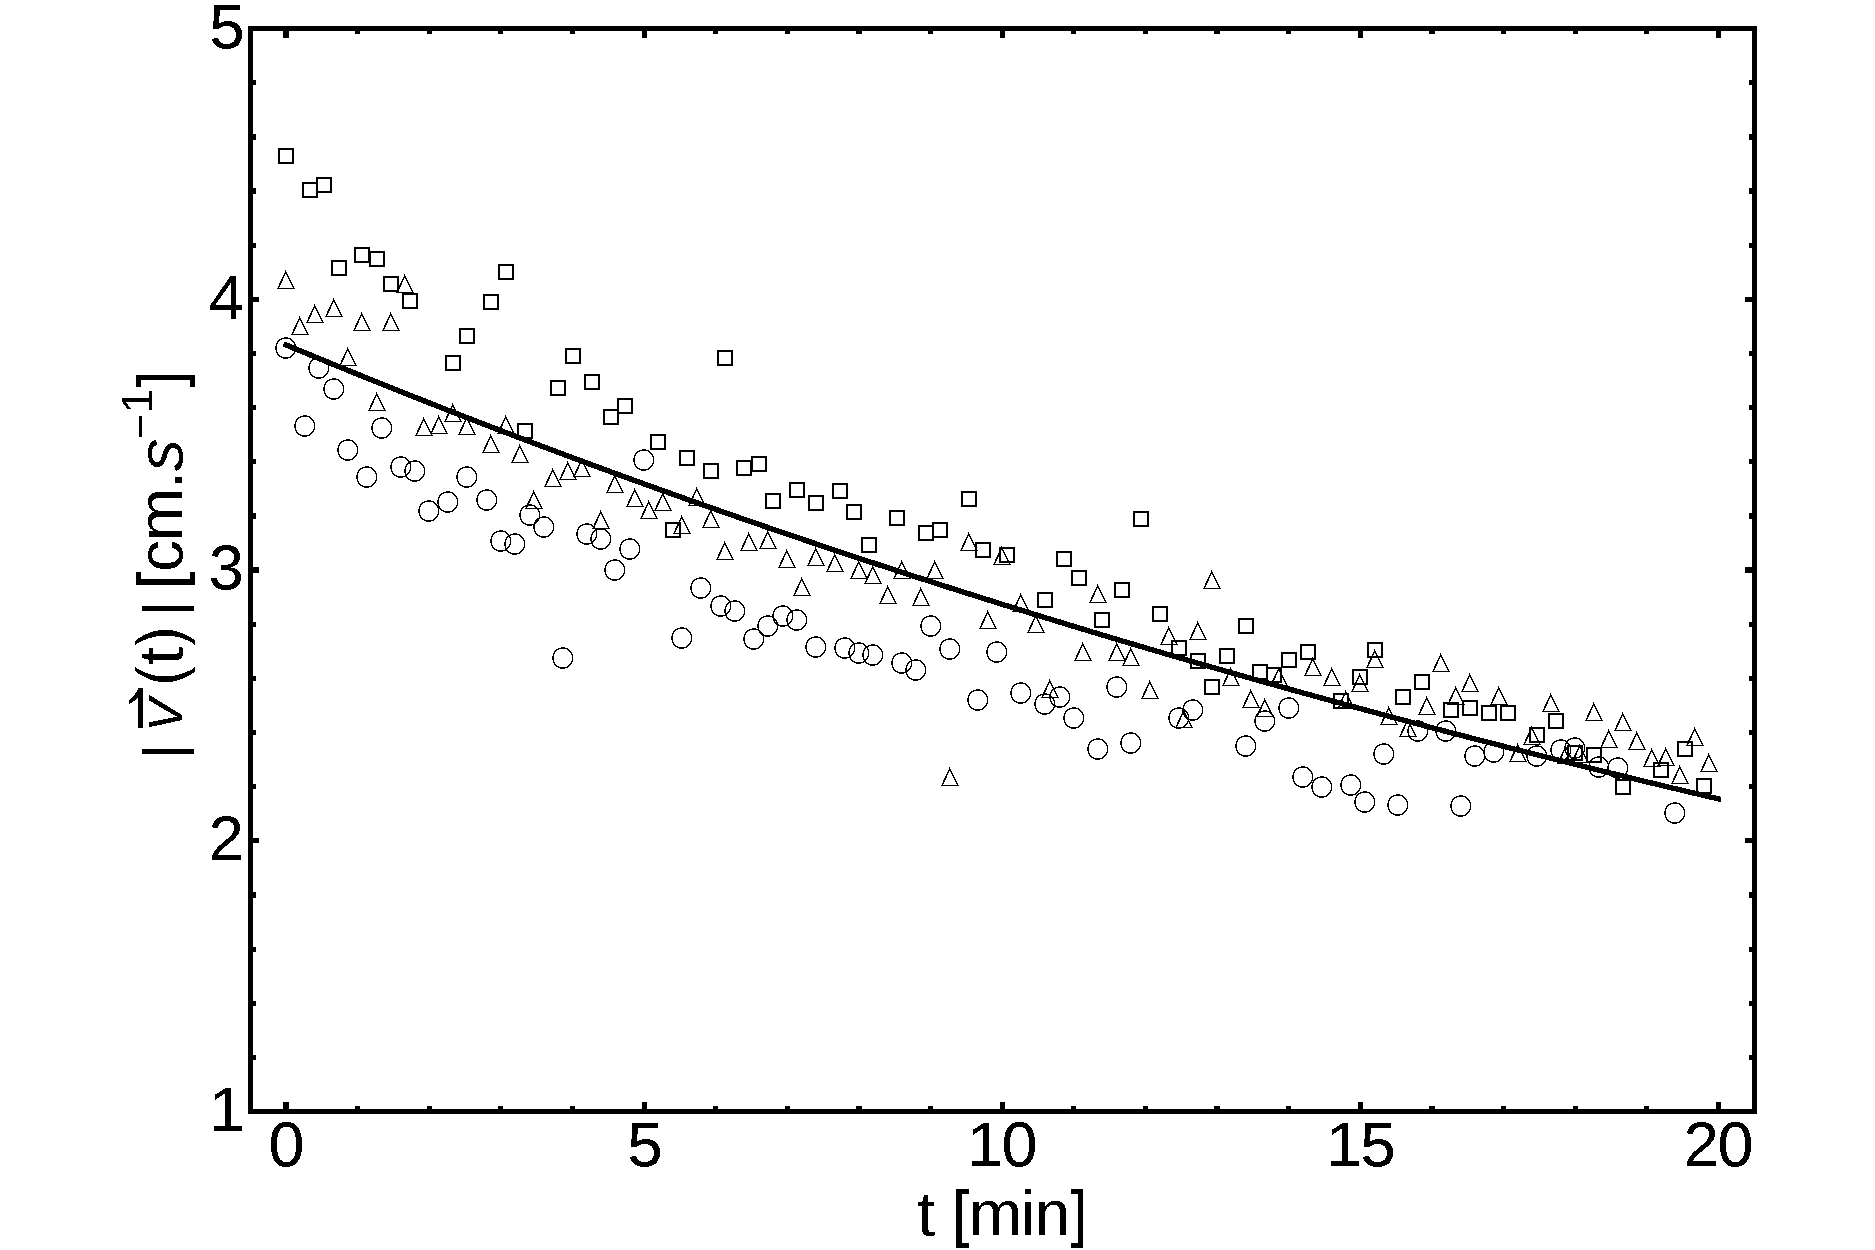
\includegraphics[scale=0.25]{lifetime.pdf}
    \end{center}
    \caption{}
    \label{fig:lifetime}
\end{figure}

\subsection{Oscillatory Motion of the cboat}
\label{sec:oscboat}
\begin{figure*}[ht]
    \centering
	\begin{minipage}[c]{0.3\linewidth}
		\centering
		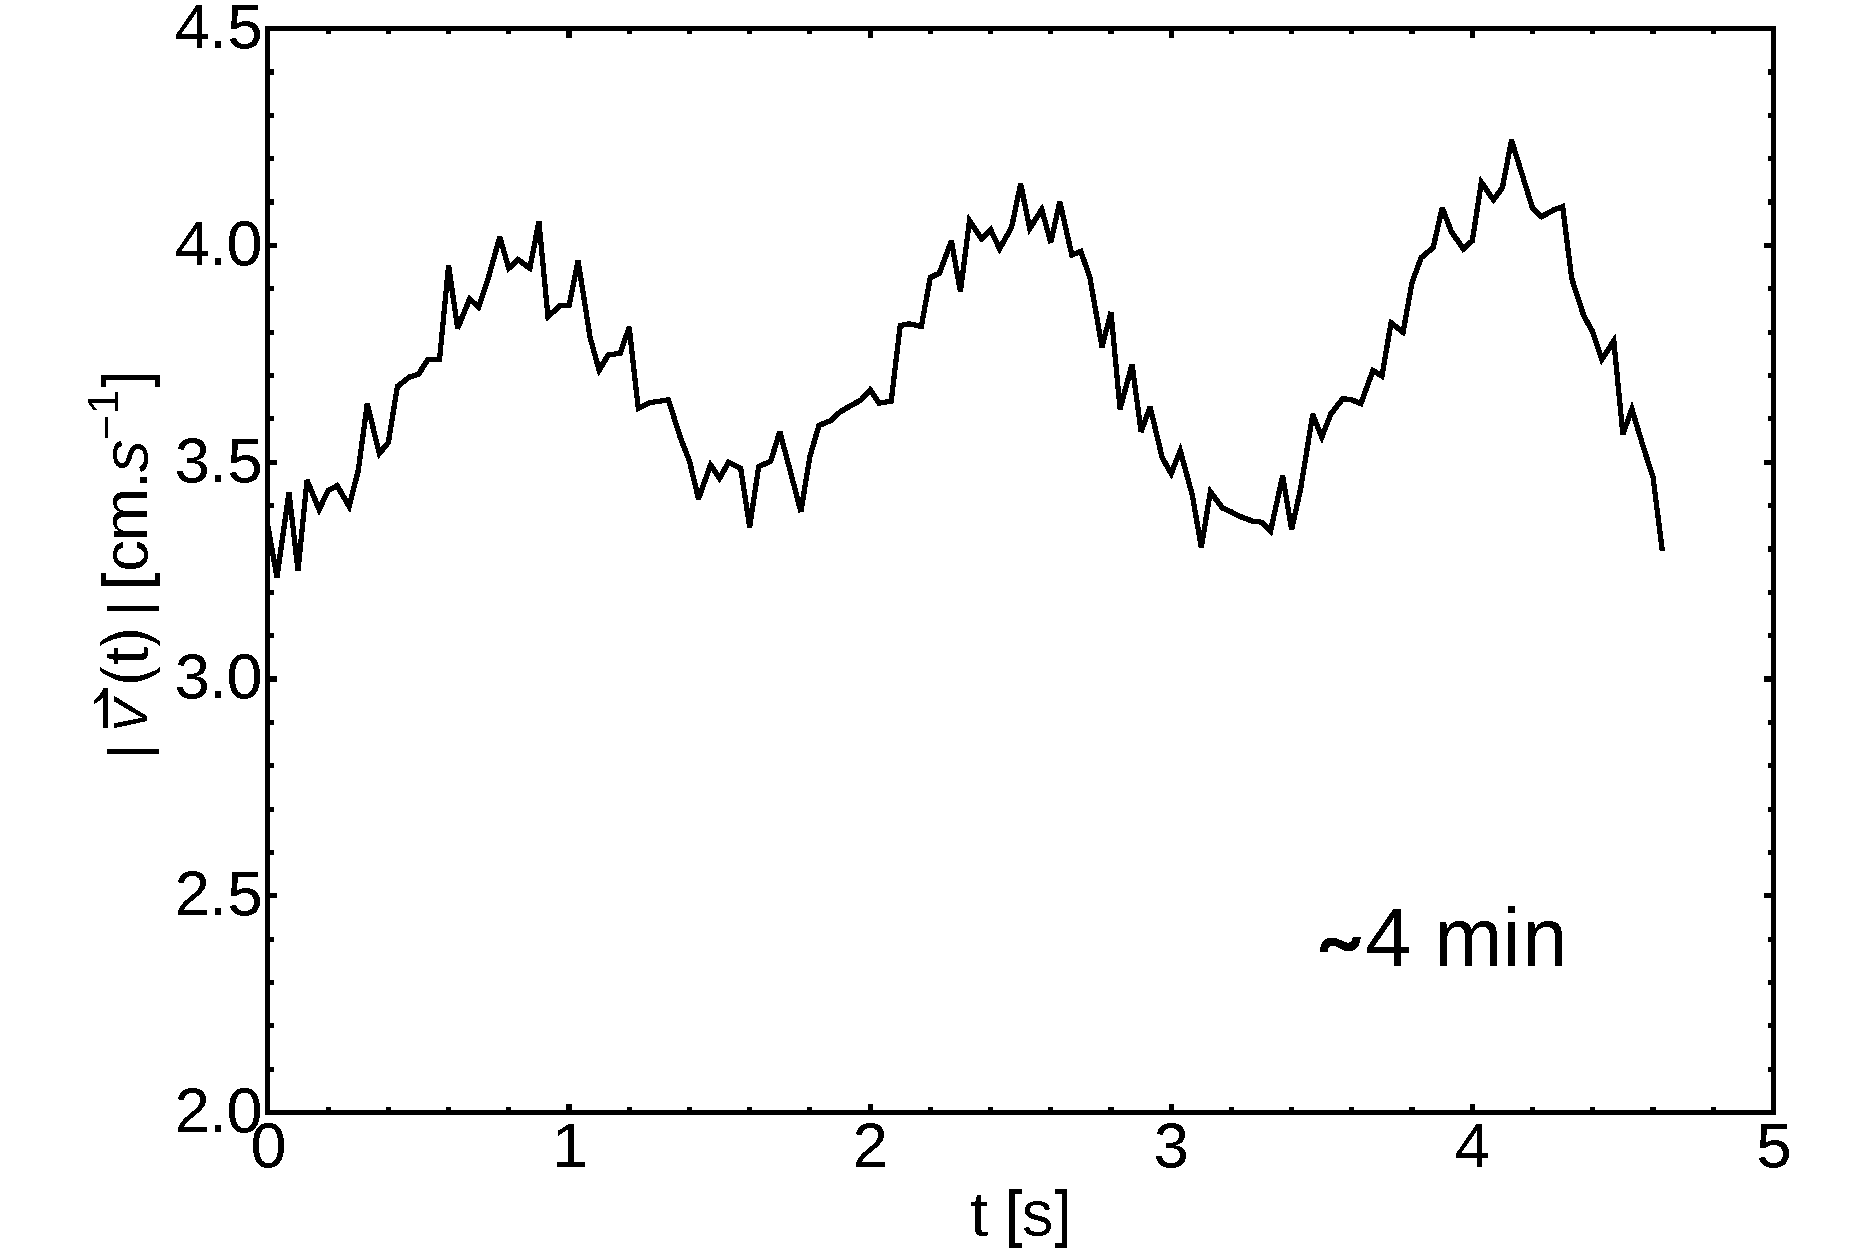
\includegraphics[width=\textwidth]{uvst_72dypcm_a.pdf}
		% \caption{$\xi > \xi_{c}$}\label{fig:uvst_72dypcm_a}		
	\end{minipage}
	\begin{minipage}[c]{0.3\linewidth}
		\centering
		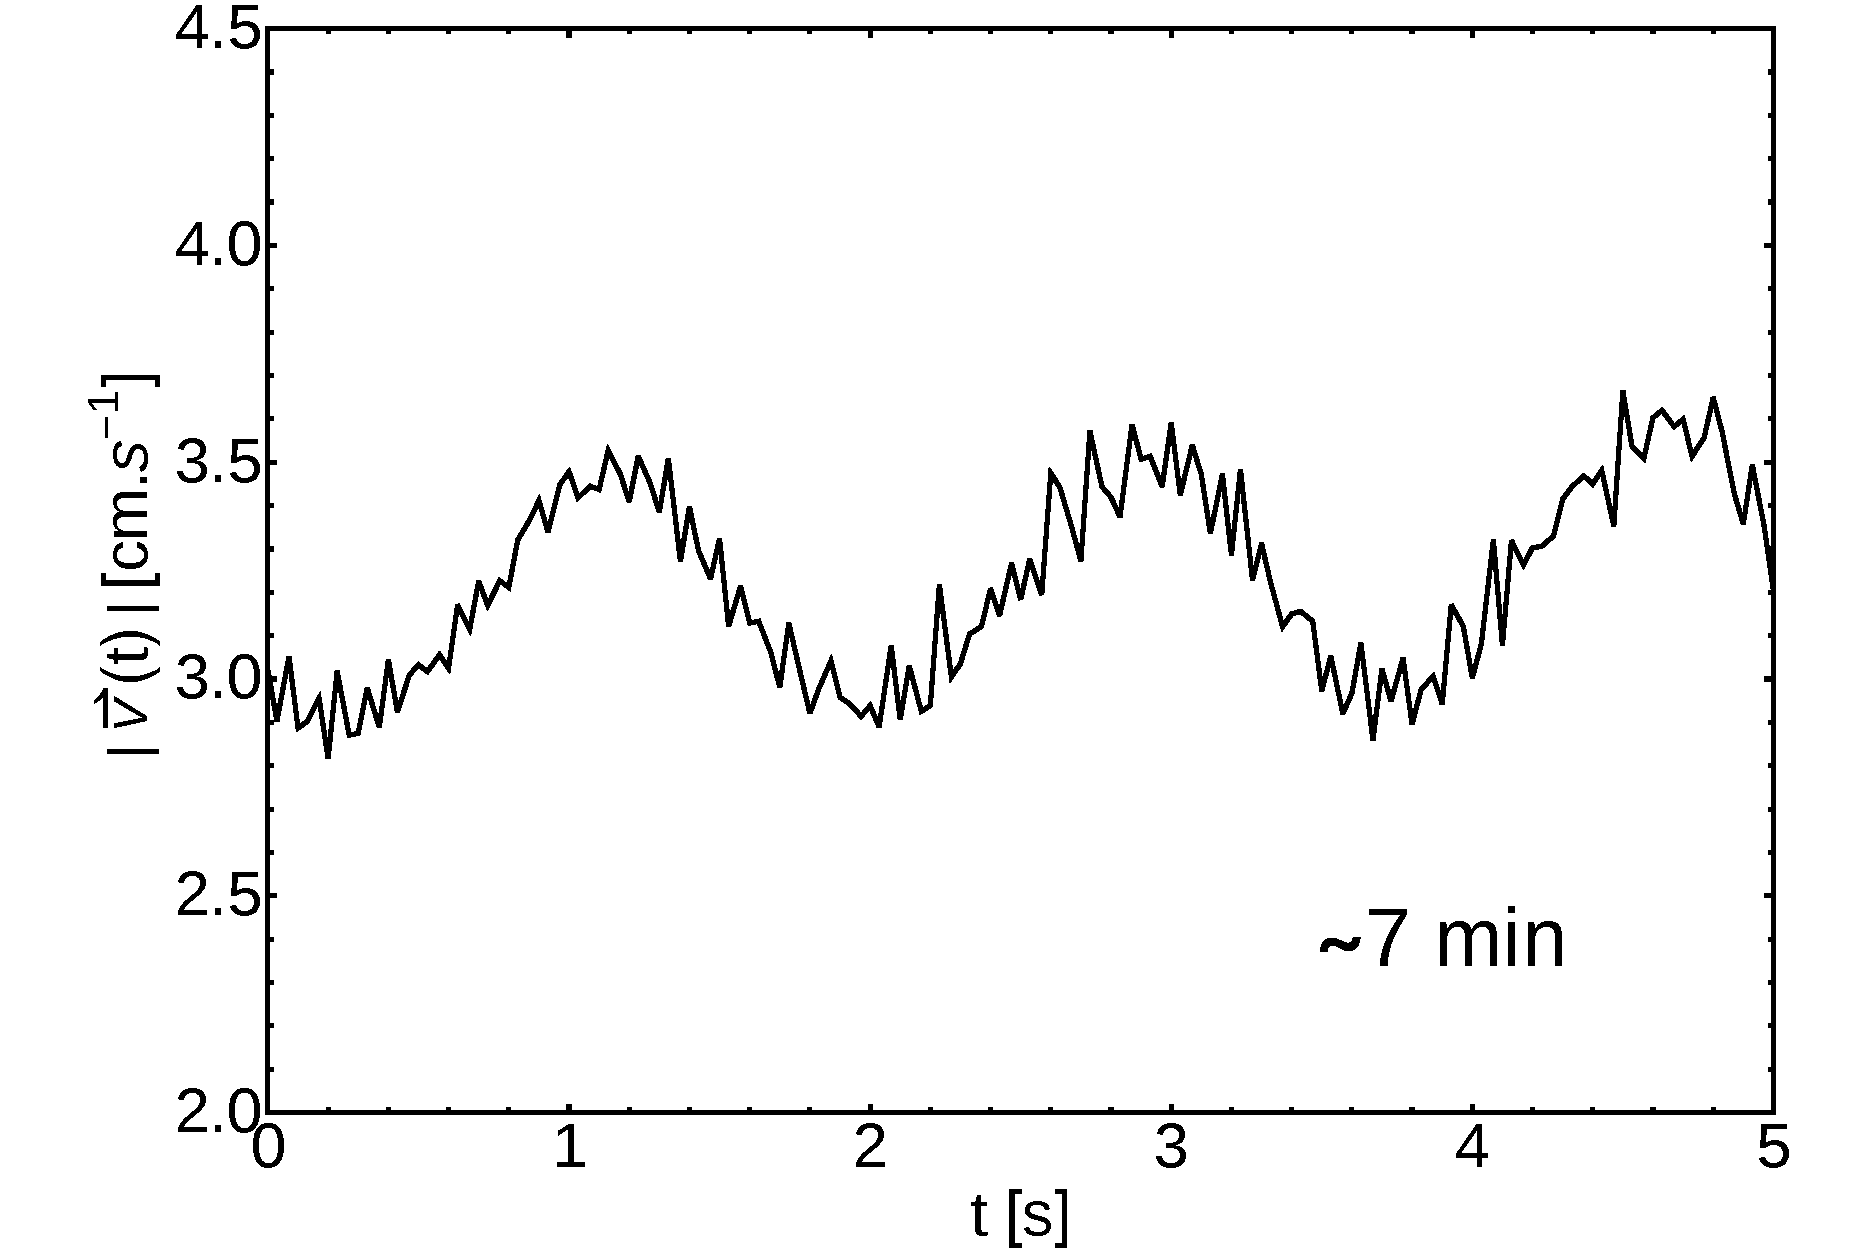
\includegraphics[width=\textwidth]{uvst_72dypcm_b.pdf}
		% \caption{$\xi > \xi_{c}$}\label{fig:uvst_72dypcm_b}
	\end{minipage}
	\begin{minipage}[c]{0.3\linewidth}
		\centering
		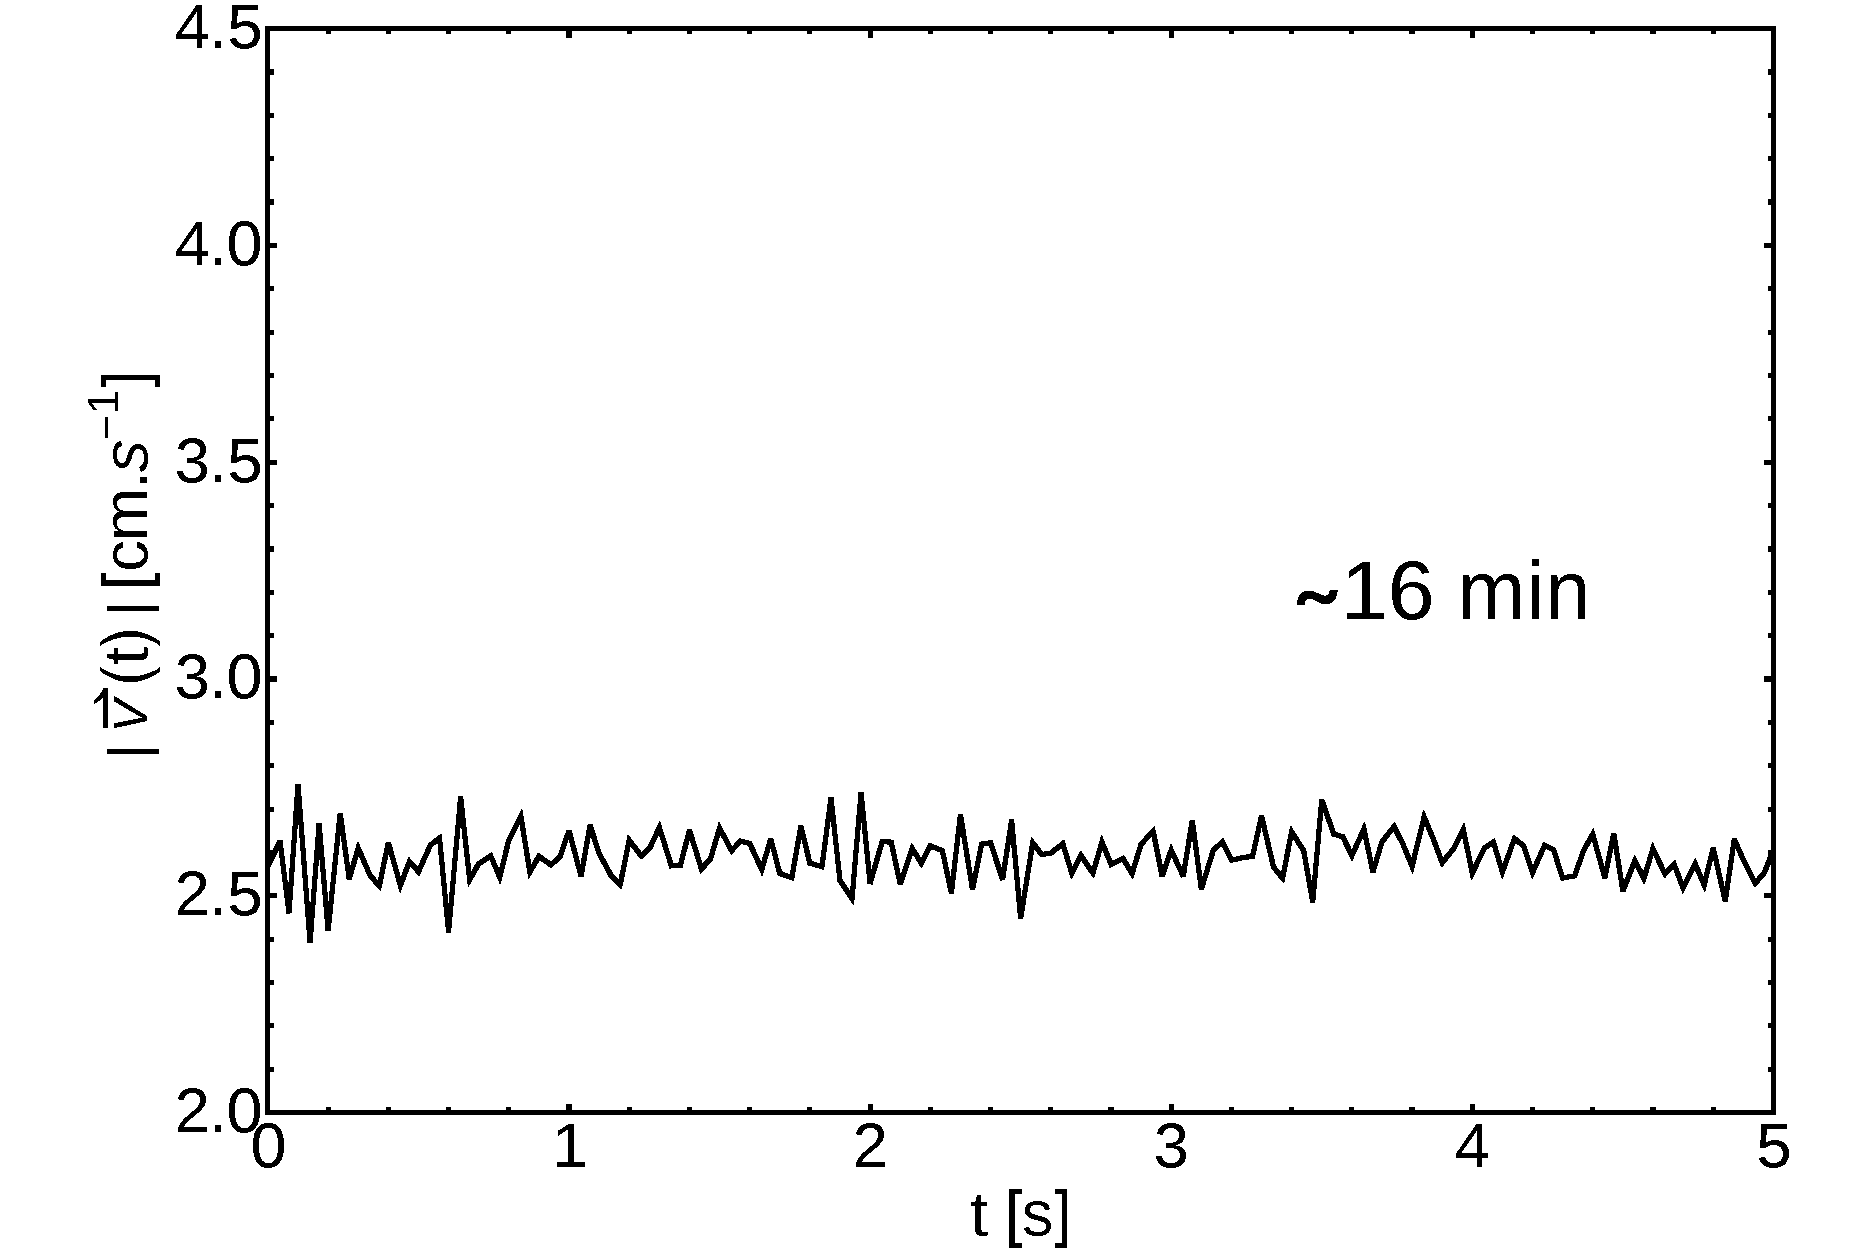
\includegraphics[width=\textwidth]{uvst_72dypcm_c.pdf}
		% \caption{$\xi \simeq \xi_{c}$}\label{fig:uvst_72dypcm_c}
	\end{minipage}
	\caption{$\xi > \xi_{c}$, $\xi > \xi_{c}$ and $\xi \simeq \xi_{c}$}\label{fig:uvst_72dypcm}
\end{figure*}
Besides the continuous decrease in speed, the cboat also exhibits oscillatory dynamics on a shorter time scale (few seconds) compared to the life time (approximately an hour) of the cboat. Figure~\ref{fig:uvst_72dypcm} shows the time traces of the cboat speed at different intervals during the course of experiment. The average speed at different intervals decreases due to the dissolution of CA in water as mentioned in previous section. The oscillations arise due to the competition between the Marangoni forces and the viscous forces. The Marangoni forces accelerate the cboat to a larger speed $u_{B}$, however the viscous forces, which scale as $u_{B}^{2}$, decelerate the cboat. As the cboat slows down, the Marangoni forces again acclerate the cboat. This driving and damping cycle leads to oscillations in cboat speed. When there is a balance between the driving and damping forces the cboat moves with terminal velocity, as shown in figure~\ref{fig:uvst_72dypcm}c. The amplitude of oscillations decreases and the period of oscillations increases (shown in figure~\ref{fig:uvst_65dypcm}) due to the dissolution of CA. In following section, we derived a dimensionless parameter $\xi$ in order to qualitatively describe the oscillatory dynamics of cboat. Furthermore, the value of $\xi$ was experimentally varied by changing the air-water interfacial tension using SDS.

The equation of motion for a cboat at the air-water interface is given by,
\begin{equation}\label{eq:eomgeneral}
\begin{aligned}
m \tdc{\mathbf{u}_{B}}{t} &= -\mathbf{F}_{D} + \oint_{C} \sigma \ \hat{\mathbf{n}} \ \td{l} \\
\mathbf{F}_{D} &\sim \rho\ a^{2} \left|\mathbf{u}_{B}\right|^{2} \hat{\mathbf{u}}_{B}
\end{aligned}
\end{equation}
where, $\mathbf{F}_{D}$ is the viscous drag acting on the cboat and $a$ is the diameter of cboat. The contour integral apperaing in equation~\ref{eq:eomgeneral} is evaluated along a circular contour of radius $R$, whose center is at the center of the cboat, and the resultant is the force acting on the cboat due to the interfacial tenion gradients. Obviously, the value of the integral is zero when surface tension gradients are symmetric. 
\begin{figure}[ht]
    \centering
	\begin{minipage}[c]{0.4\linewidth}
		\centering
		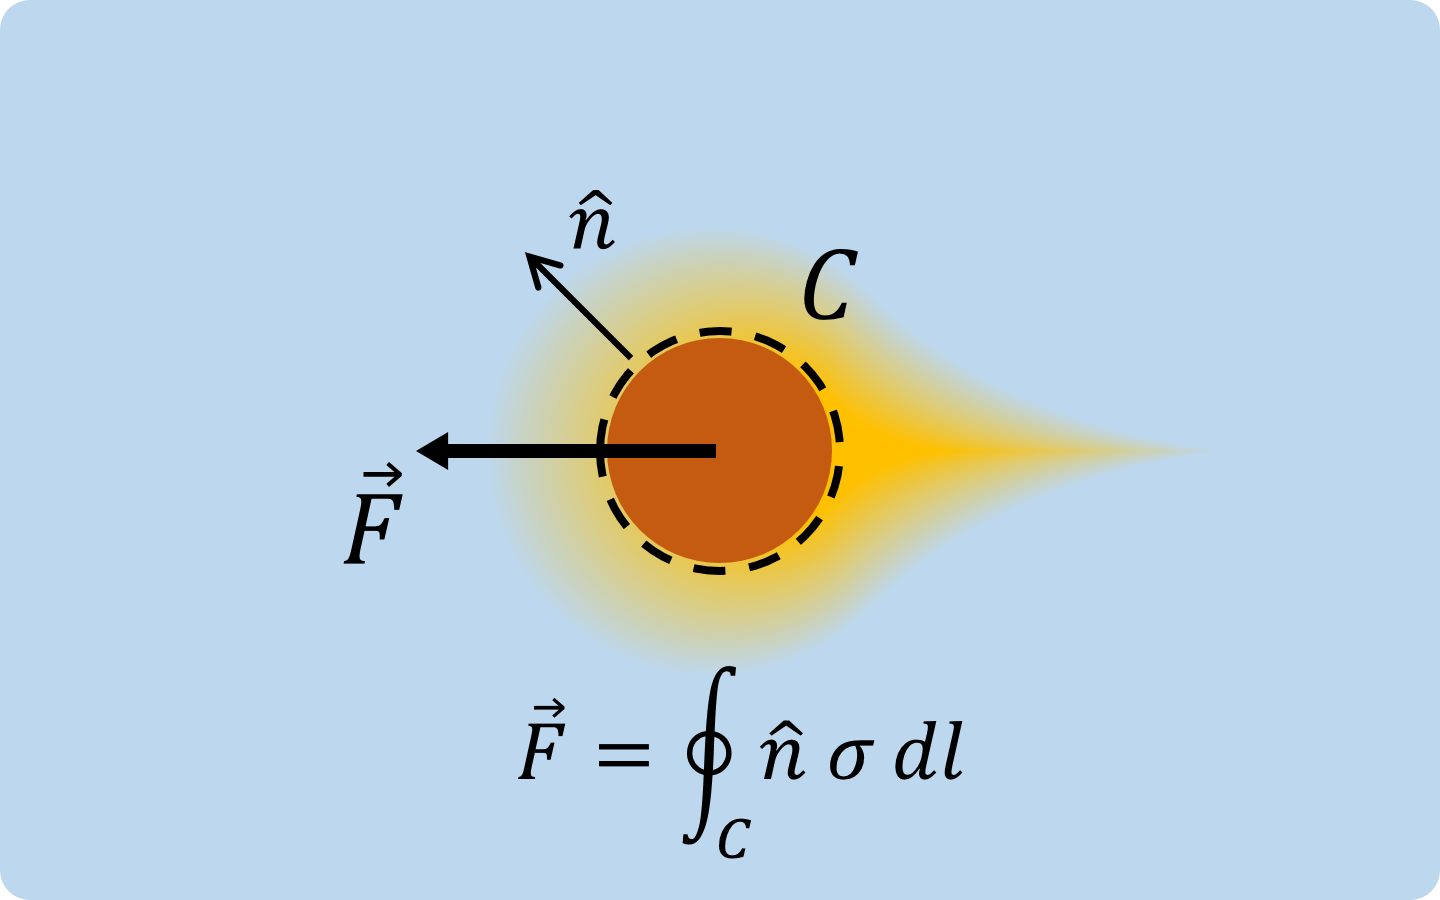
\includegraphics[width=\textwidth]{schematic_a_v1.png}
		% \caption{Top view}\label{fig:schem_top}		
	\end{minipage}
	\begin{minipage}[c]{0.4\linewidth}
		\centering
		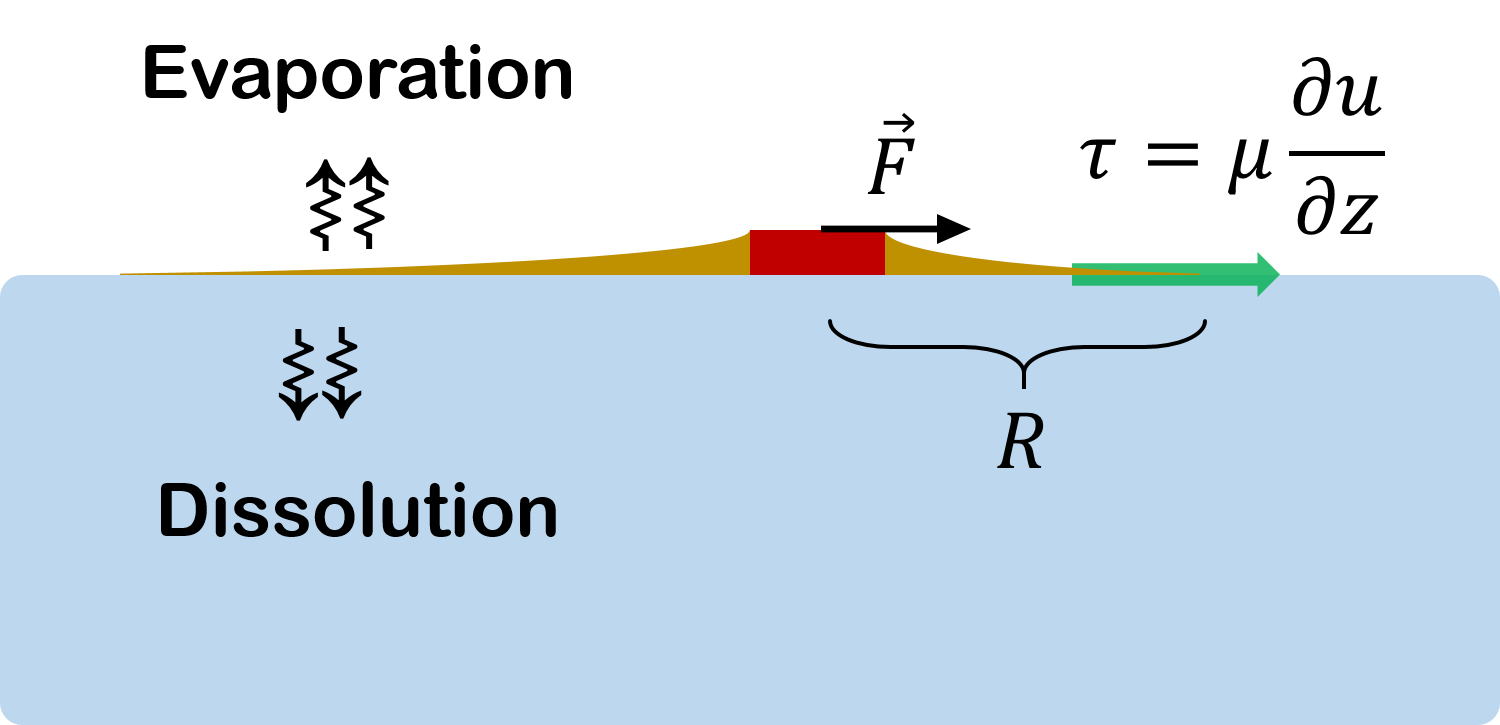
\includegraphics[width=\textwidth]{schematic_b_v1.png}
		% \caption{Side view}\label{fig:schem_side}
	\end{minipage}
	\caption{Schematic of cboat in motion (a) top view (b) side view obtained along a horizontal line bisecting the cboat and along the direction of motion. Viscous drag \emph{not} shown in schematic. In case of CA, evaporation/sublimation is negligible in comparison to dissolution.}\label{fig:schematic}
\end{figure}
\subsubsection{Estimation of cboat velocity scale}
For brevity, let us assume that the cboat exhibits rectilinear motion then the set of equations~\ref{eq:eomgeneral} simplifies to
\begin{equation}
m \tdc{u_{B}}{t} \simeq -\rho\ a^{2}\ u_{B}^{2} + \Delta\sigma\ a
\end{equation}
where, $\Delta\sigma$ is the interfacial tension difference in forward (or CA poor region) and backward (or CA rich region) directions of the cboat. We can obtain a scaling for the average speed, $U_{B}$ of the cboat as, 
\begin{align}
0 &\simeq -\rho\ a^{2}\ U_{B}^{2} + \Delta\sigma\ a  \nonumber \\
\implies U_{B} &\simeq \sqrt{\frac{\Delta\sigma}{\rho a}} 
\end{align}
Note that, the cboat velocity does not depend on the viscosity of the fluid because for the cboat system the Reynolds number is $\simeq 100$.
\subsubsection{Marangoni and Reynolds numbers for the fluid flow}
% When the cboat is held fixed at the air-water interface, symmetric CA concentration gradients are set up around the cboat.
At the air-water interface, the shear stress caused by the interfacial tension gradients shear the air-water interface causing the underlying fluid flow. The shear stress is balanced by the viscous stress (figure~\ref{fig:schematic}b).
\begin{equation*}
\tau = \mu \pdc{u_{M}}{z} 
\implies \pdc{\sigma}{x} = \mu \pdc{u_{M}}{z}
\end{equation*} 
where, $u_{M}$ is the fluid velocity at the air-water interface. The Marangoni number, $\mathtt{Ma}$ which is defined as the ratio of interfacial tension forces and viscous forces, is given by
\begin{equation}\label{eq:numberMa}
\mathtt{Ma} = \frac{\Delta\sigma\ \delta}{U_{M} \mu L}
\end{equation}
where, $\frac{\Delta\sigma}{L}$ is the interfacial tension gradient shearing the interface over the length, $L$ of the interface, $U_{M}$ is the characteristic flow velocity, $\delta$ is the boundary layer thickness and $\mu$ is the dynamic viscosity of the fluid. The Reynolds number, $\mathtt{Re}$ corresponding to the fluid flow is given by,
\begin{equation}\label{eq:numberRe}
\mathtt{Re} = \frac{\rho U_{M} L}{\mu}
\end{equation}
Obtaining a scaling expression for the flow velocity, $U_{M}$ is cumbersome; instead one can eliminate $U_{M}$ by multiplying $\mathtt{Ma}$ and $\mathtt{Re}$, which yields,
\begin{equation}
\mathtt{Ma} \cdot \mathtt{Re} = \frac{\Delta\sigma\ \rho}{\mu^{2}} \delta = \frac{\delta}{l_{M}}
\end{equation}
where, $l_{M} = \frac{\mu^{2}}{\Delta\sigma\ \rho}$ is defined as the Marangoni characteristic length scale. %In order to achieve Marangoni flow, $\mathtt{Ma} \sim 1$ and the flow to be laminar $\mathtt{Re} < 1$, which implies the boundary layer thickness, $\delta < l_{M}$ the Marangoni characteristic length scale. 
\subsubsection{Dimensionless parameter, $\xi$}
We can define a dimensionless parameter using the natural length scales in the system Marangoni characteristic length, $l_{M}$ and the diameter of the cboat, $a$
\begin{equation}
\xi = \frac{a}{l_{M}} = \frac{\Delta\sigma\rho\ a}{\mu^{2}}
\end{equation}
\begin{figure*}[ht]
    \centering
	\begin{minipage}[c]{0.3\linewidth}
		\centering
		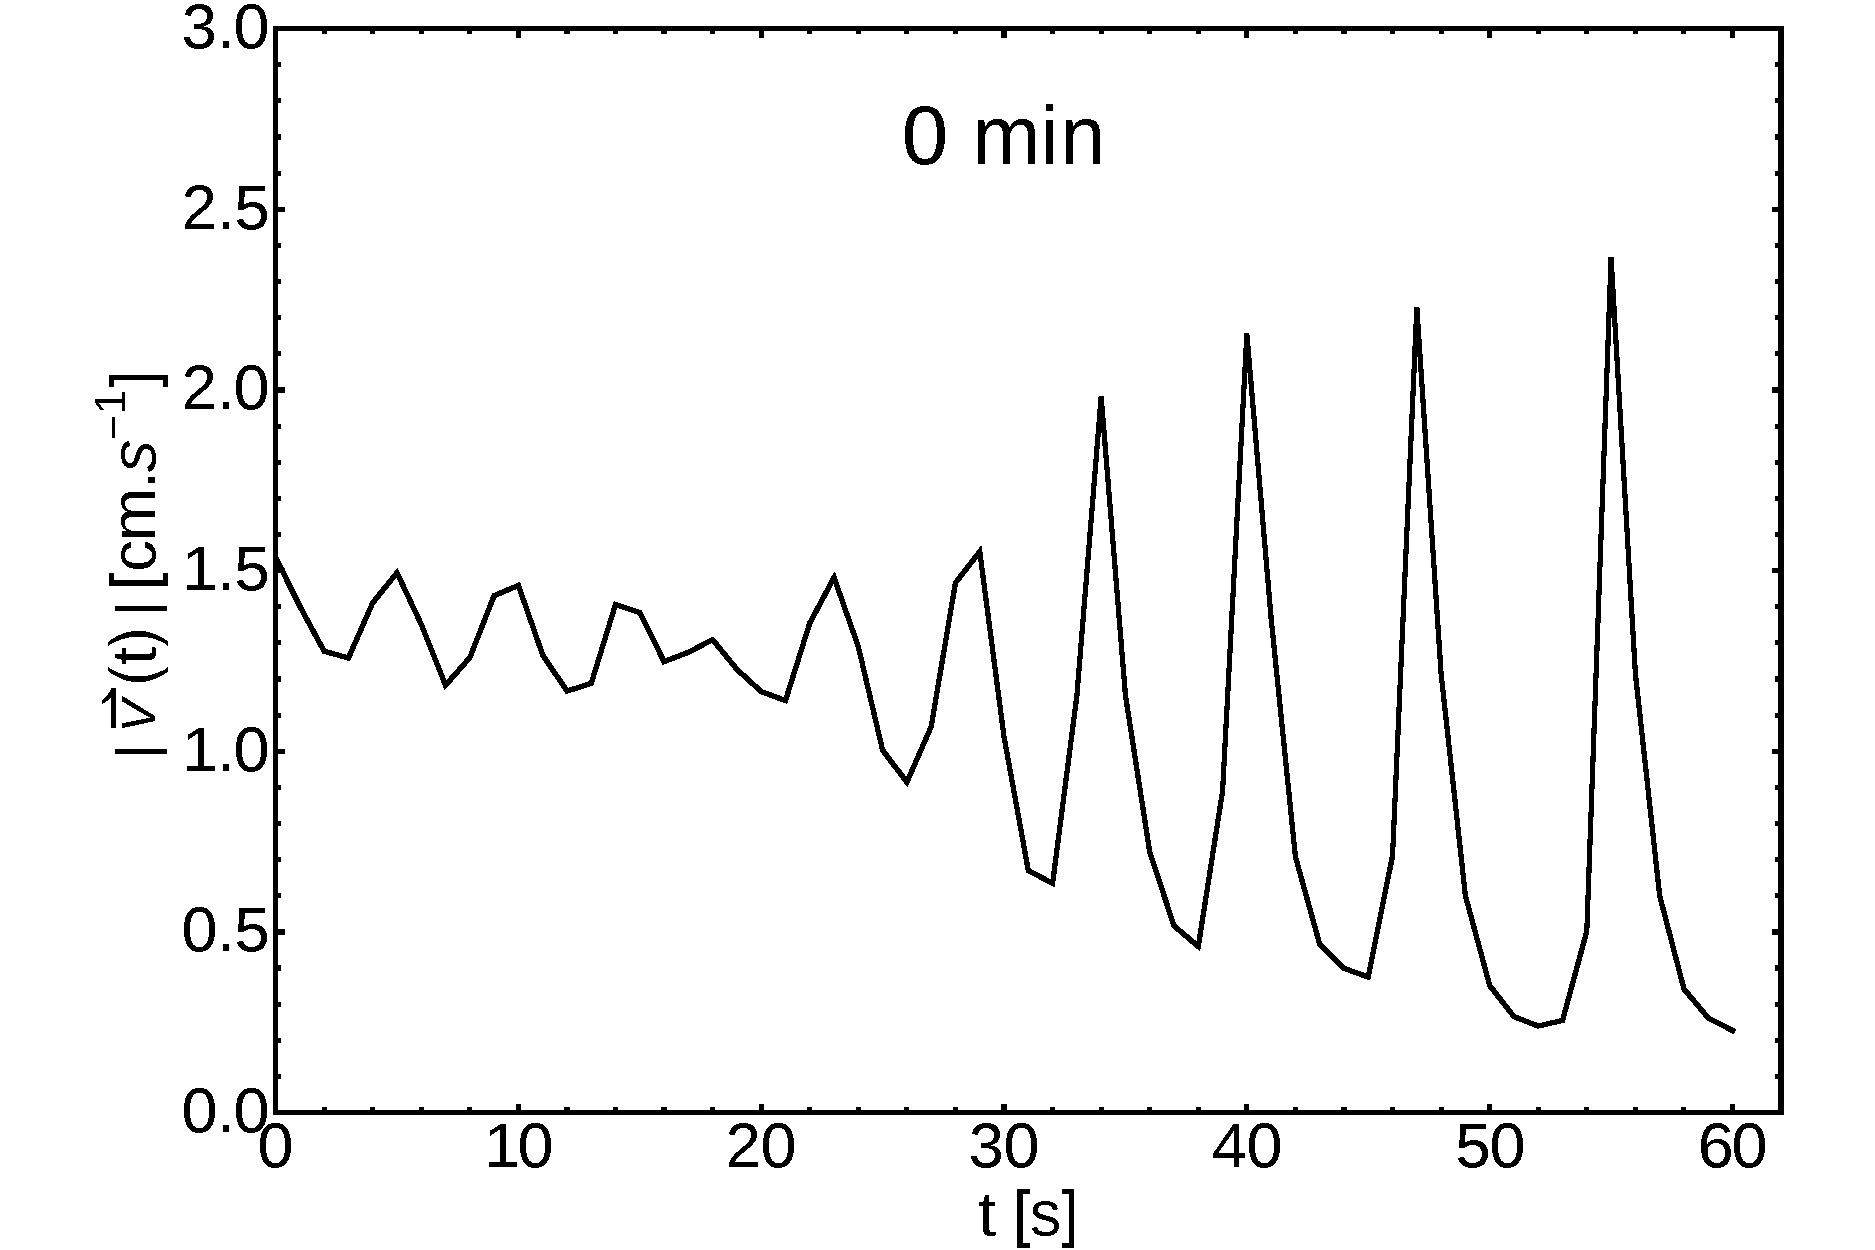
\includegraphics[width=\textwidth]{uvst_65dypcm_a.pdf}
		% \caption{$\xi \simeq \xi_{c}$}\label{fig:uvst_65dypcm_a}		
	\end{minipage}
	\begin{minipage}[c]{0.3\linewidth}
		\centering
		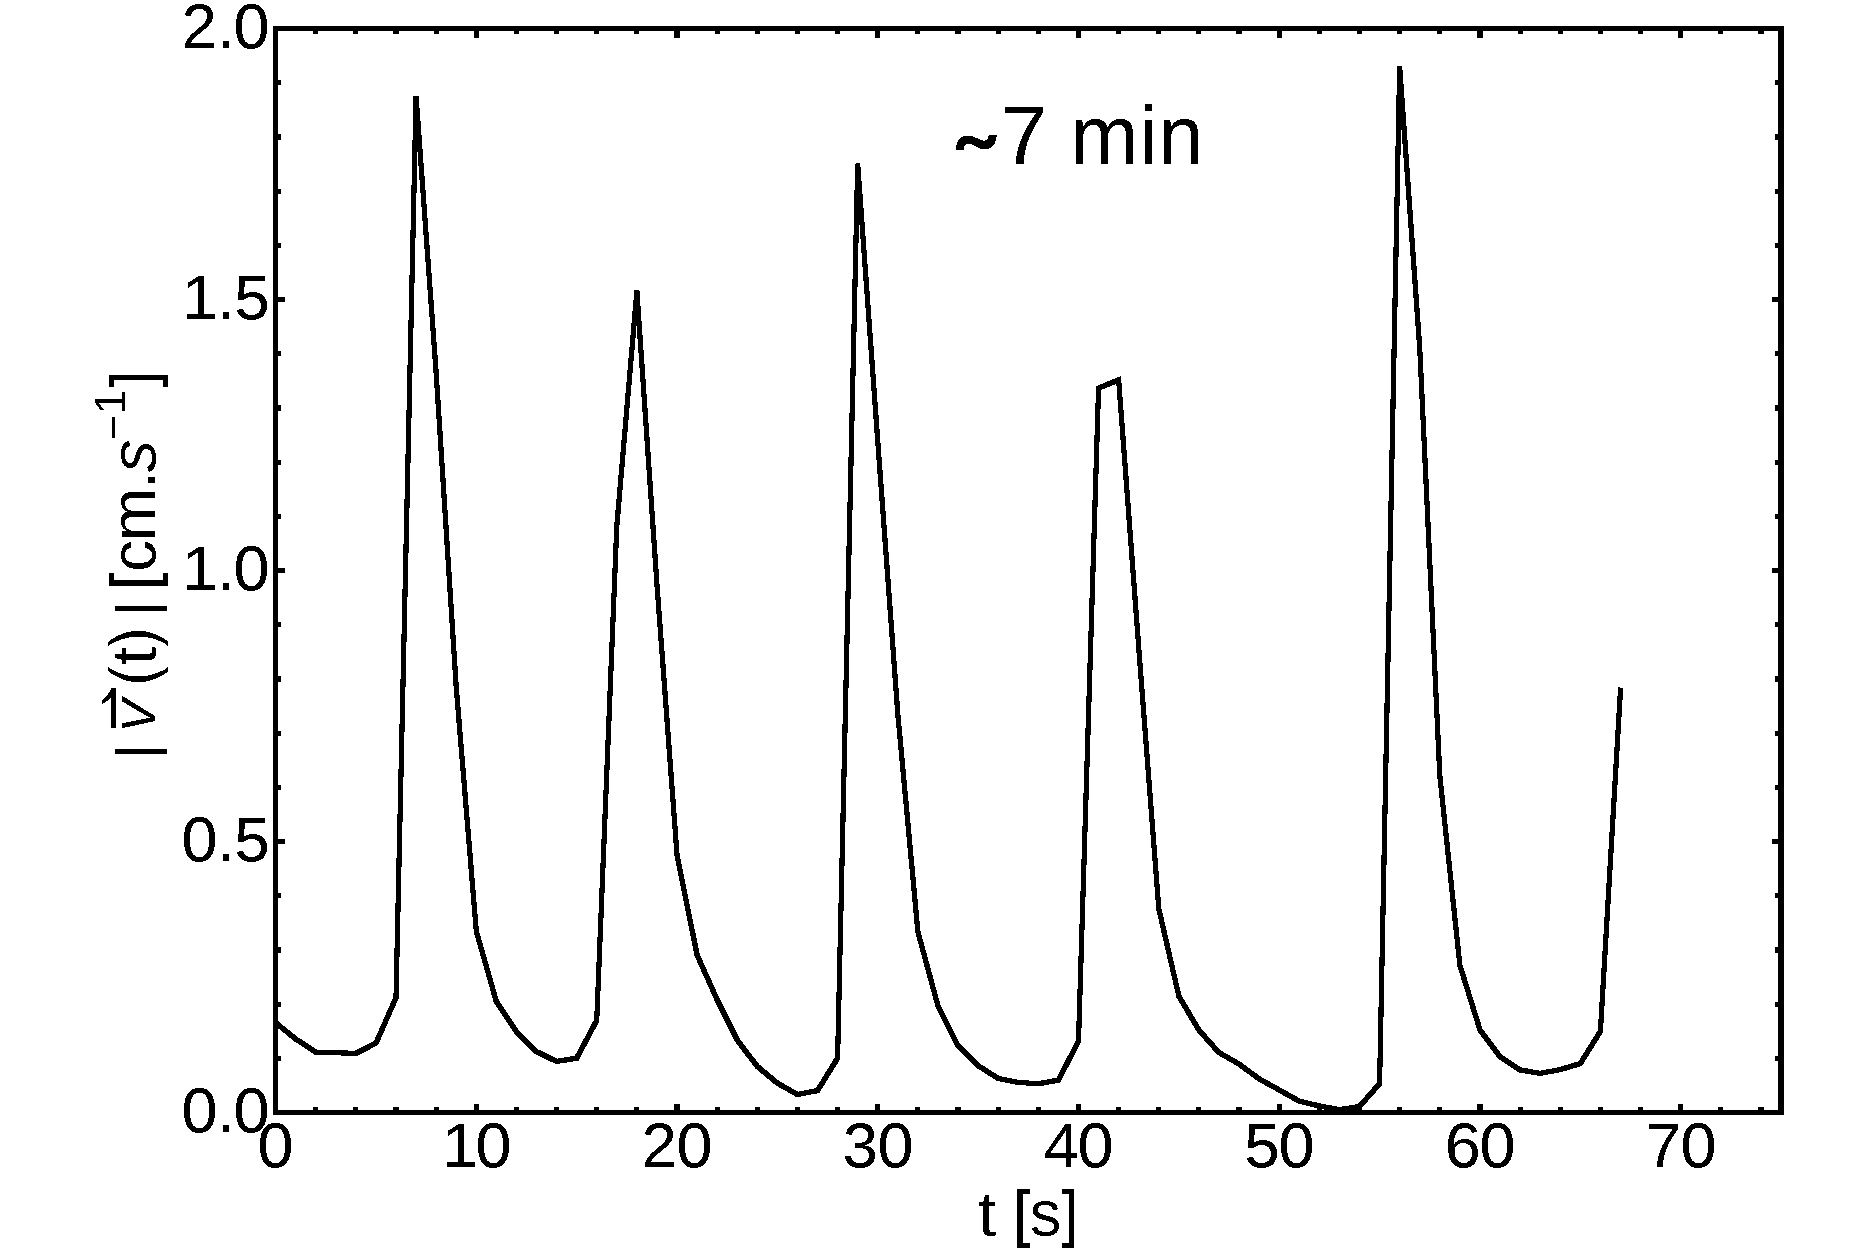
\includegraphics[width=\textwidth]{uvst_65dypcm_b.pdf}
		% \caption{$\xi < \xi_{c}$}\label{fig:uvst_65dypcm_b}
	\end{minipage}
	\begin{minipage}[c]{0.3\linewidth}
		\centering
		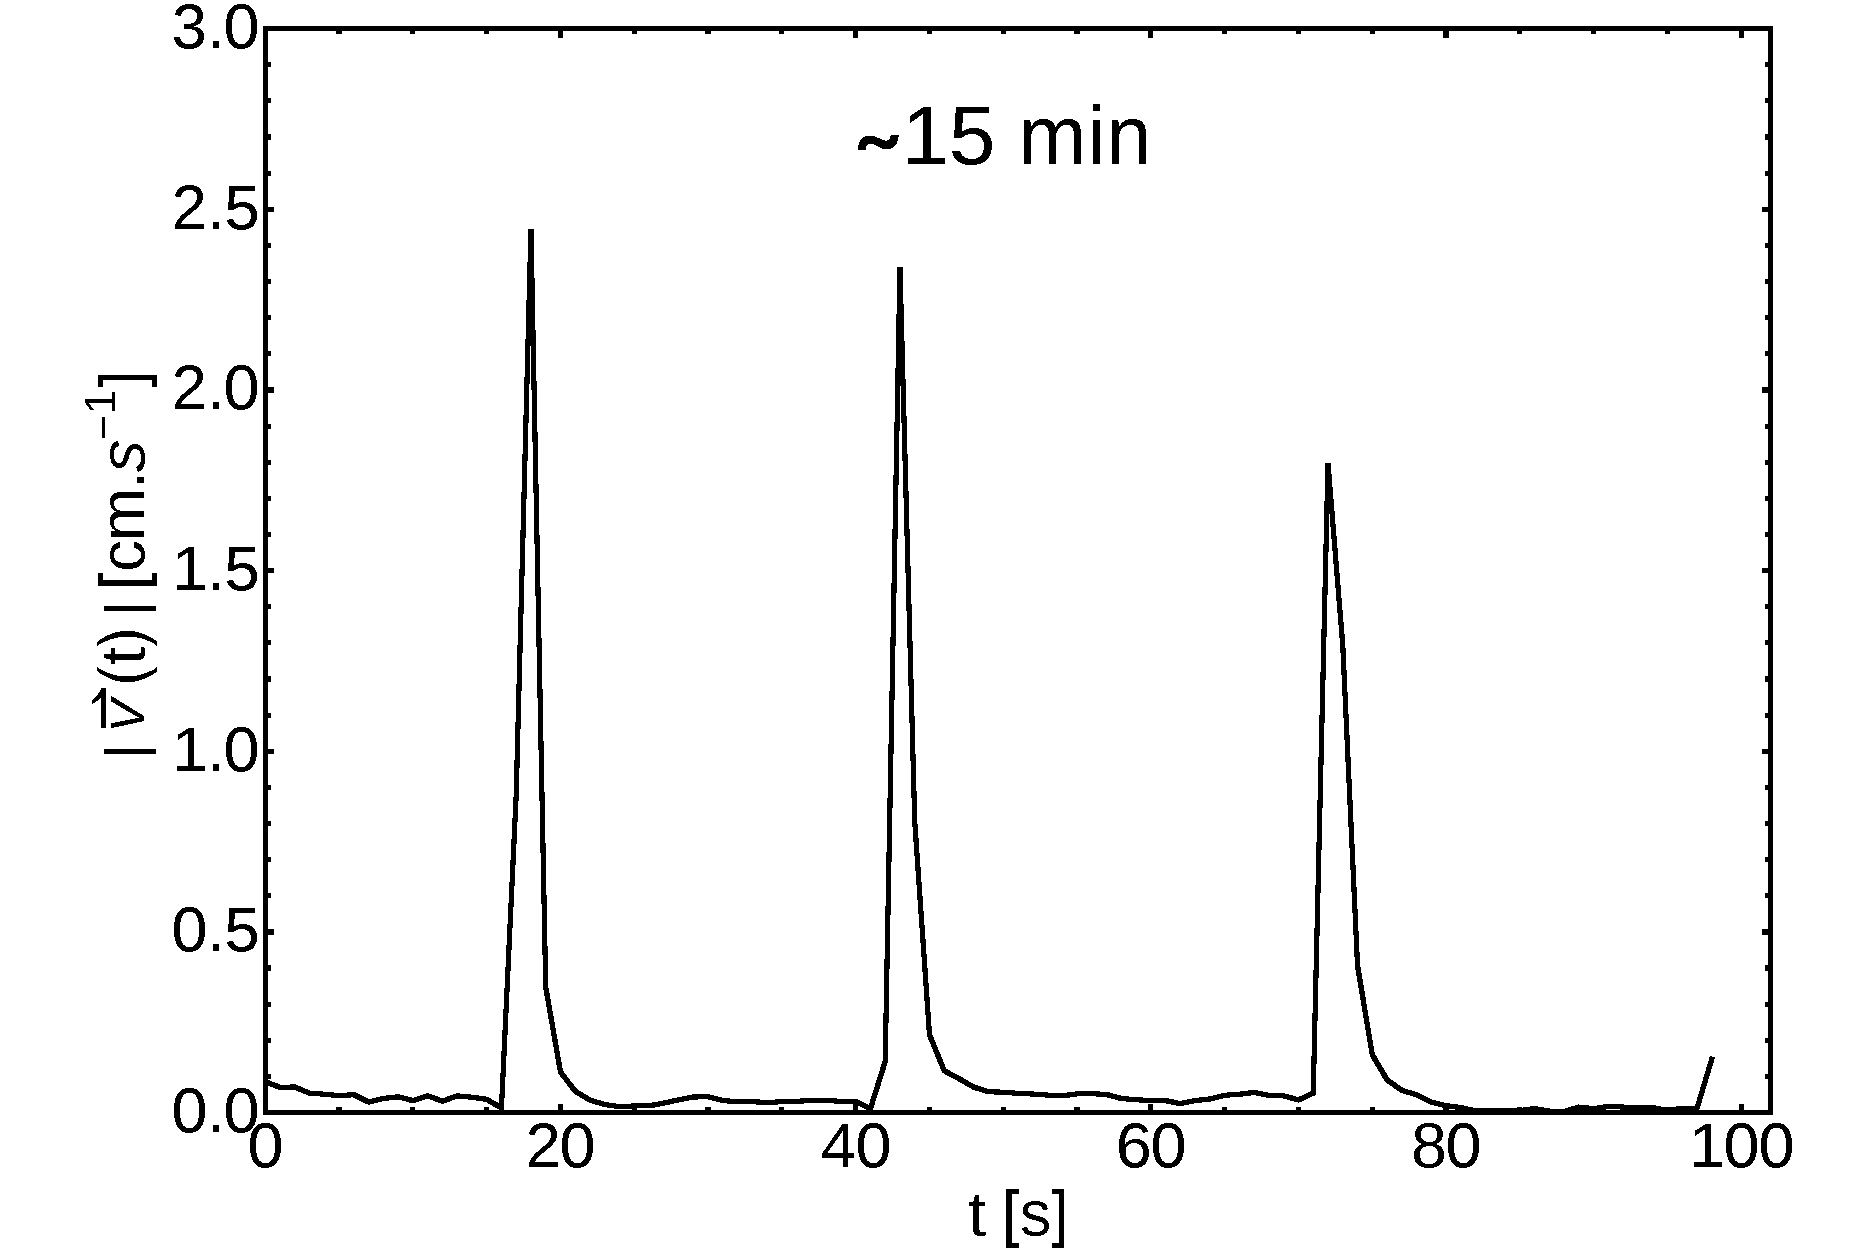
\includegraphics[width=\textwidth]{uvst_65dypcm_c.pdf}
		% \caption{$\xi << \xi_{c}$}\label{fig:uvst_65dypcm_c}
	\end{minipage}
	\caption{$\xi \simeq \xi_{c}$, $\xi < \xi_{c}$ and $\xi << \xi_{c}$}\label{fig:uvst_65dypcm}
\end{figure*}
\begin{figure}[ht] 
    \begin{center}
       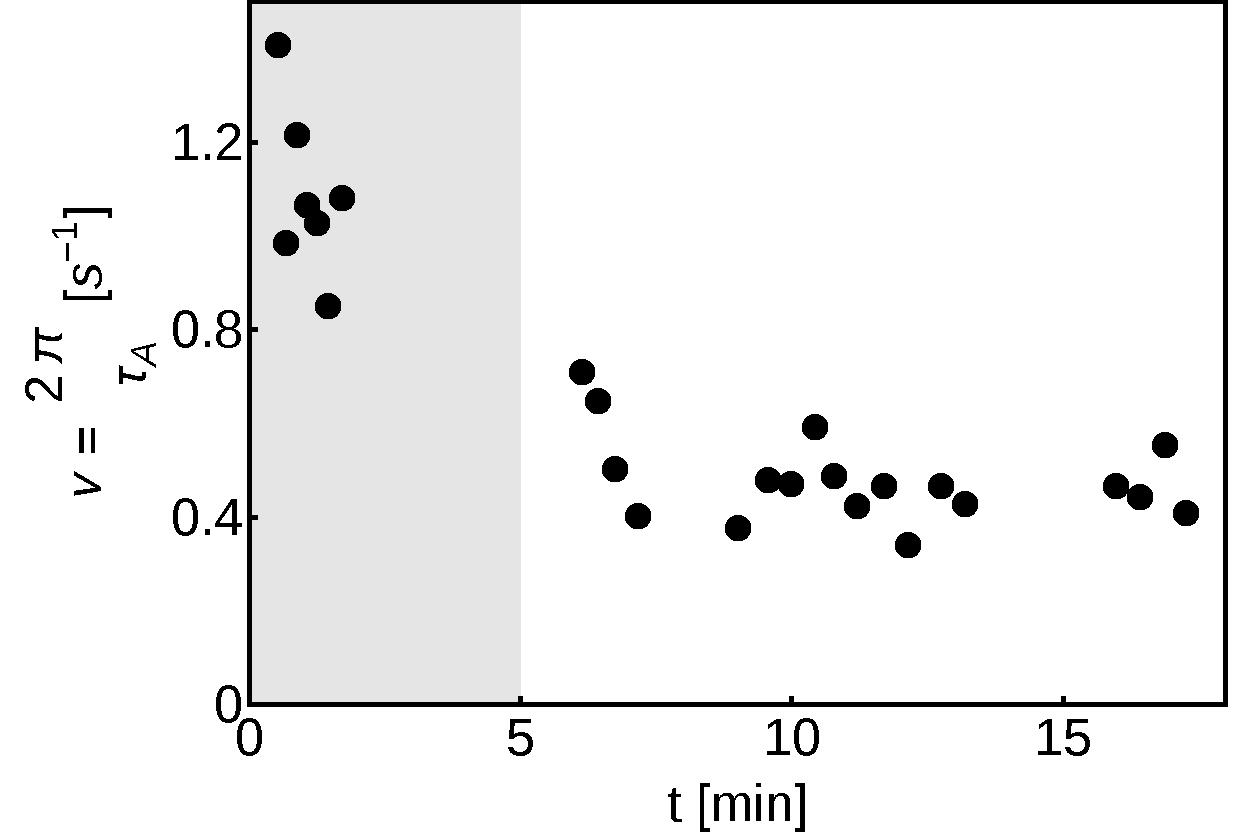
\includegraphics[scale=0.4]{freqvst.pdf}
    \end{center}
    \caption{Frequency of oscillation vs. time. Grayed out area is the transient phase during which excess CA present on the surface of the cboat.}
    \label{fig:freqvst}
\end{figure}

We \emph{define} a critical value $\xi_{c}$ for the parameter $\xi$ at which the cboat moves with terminal velocity. The critical value $\xi_{c} \simeq 5625$ is estimated from the experimental data in figure~\ref{fig:uvst_72dypcm}c. \par
Naturally, the dimensionless parameter, $\xi$ constantly decreases during the expriment due to the dissolution of CA in water. However, we varied $\xi$ by modifying the air-water interfacial tension using SDS. Figure~\ref{fig:uvst_65dypcm} shows the speed traces of a cboat at different intervals of time when the air-water interfacial tension is decreased to $65\ \mathrm{dy/cm}$. We observe that, the average speed of the cboat at different intervals decreases and the period of the oscillations increases. Another subtle observation is the distance travelled by the cboat, given by the area under the speed vs. time curves, between oscillations is approximately equals to the distance, $R$ out to which CA molecules are spread by the Marangoni flow and beyond $R$, CA concentration is zero due to dissolution. During the course of experiment $R$ constantly decreases due to dissolution of CA in water. The period of oscillation is governed by the advection time scale, $\tau_{A} \sim \frac{R}{U_{M}}$, which is the time taken by a CA molecule to get advected from the periphery of the cboat to a distance $R$ and $U_{M}$ is the Marangoni flow velocity. Figure~\ref{fig:freqvst} shows the frequency of oscillation $\nu = \frac{2\pi}{\tau_{A}}$ during the course of the experiment performed at $\sigma = 65\ \mathrm{dy/cm}$. The grayed out region is the transient phase which is a result of quick dissolution of CA particles which are loosely adhered to the surface of cboat i.e. which are not embedded in the gel matrix. Past the transient phase, frequency of oscillation constantly decreases due to dissolution of CA in water. Since the cboat is mostly not moving (figure~\ref{fig:uvst_65dypcm}) during the course of the experiment the dissolution rate is solely limited by diffusion of CA molecules in water considerably increasing the life time of cboat in comparison to a constantly moving cboat (figure~\ref{fig:uvst_72dypcm}). As a result we don't observe considerable change in the frequency during the course of the experiment. When the air-water interfacial tension is decreased to such an extent beyond which dissolution of CA in water has \emph{no} effect on the air-water interfacial results in \emph{no} motion of cboat. Figure~\ref{fig:uvst_sigma} shows the plots of cboat speed versus time at different air-water interfacial tensions. As shown in figure~\ref{fig:uvst_sigma}c, when $\sigma = 59\ \mathrm{dy/cm}$, cboat's motion ceases; note that the obseved non-zero speed is due to the drift of cboat because ambient fluctuations.   
\begin{figure*}[ht]
    \centering
	\begin{minipage}[t]{0.3\linewidth}
		\centering
		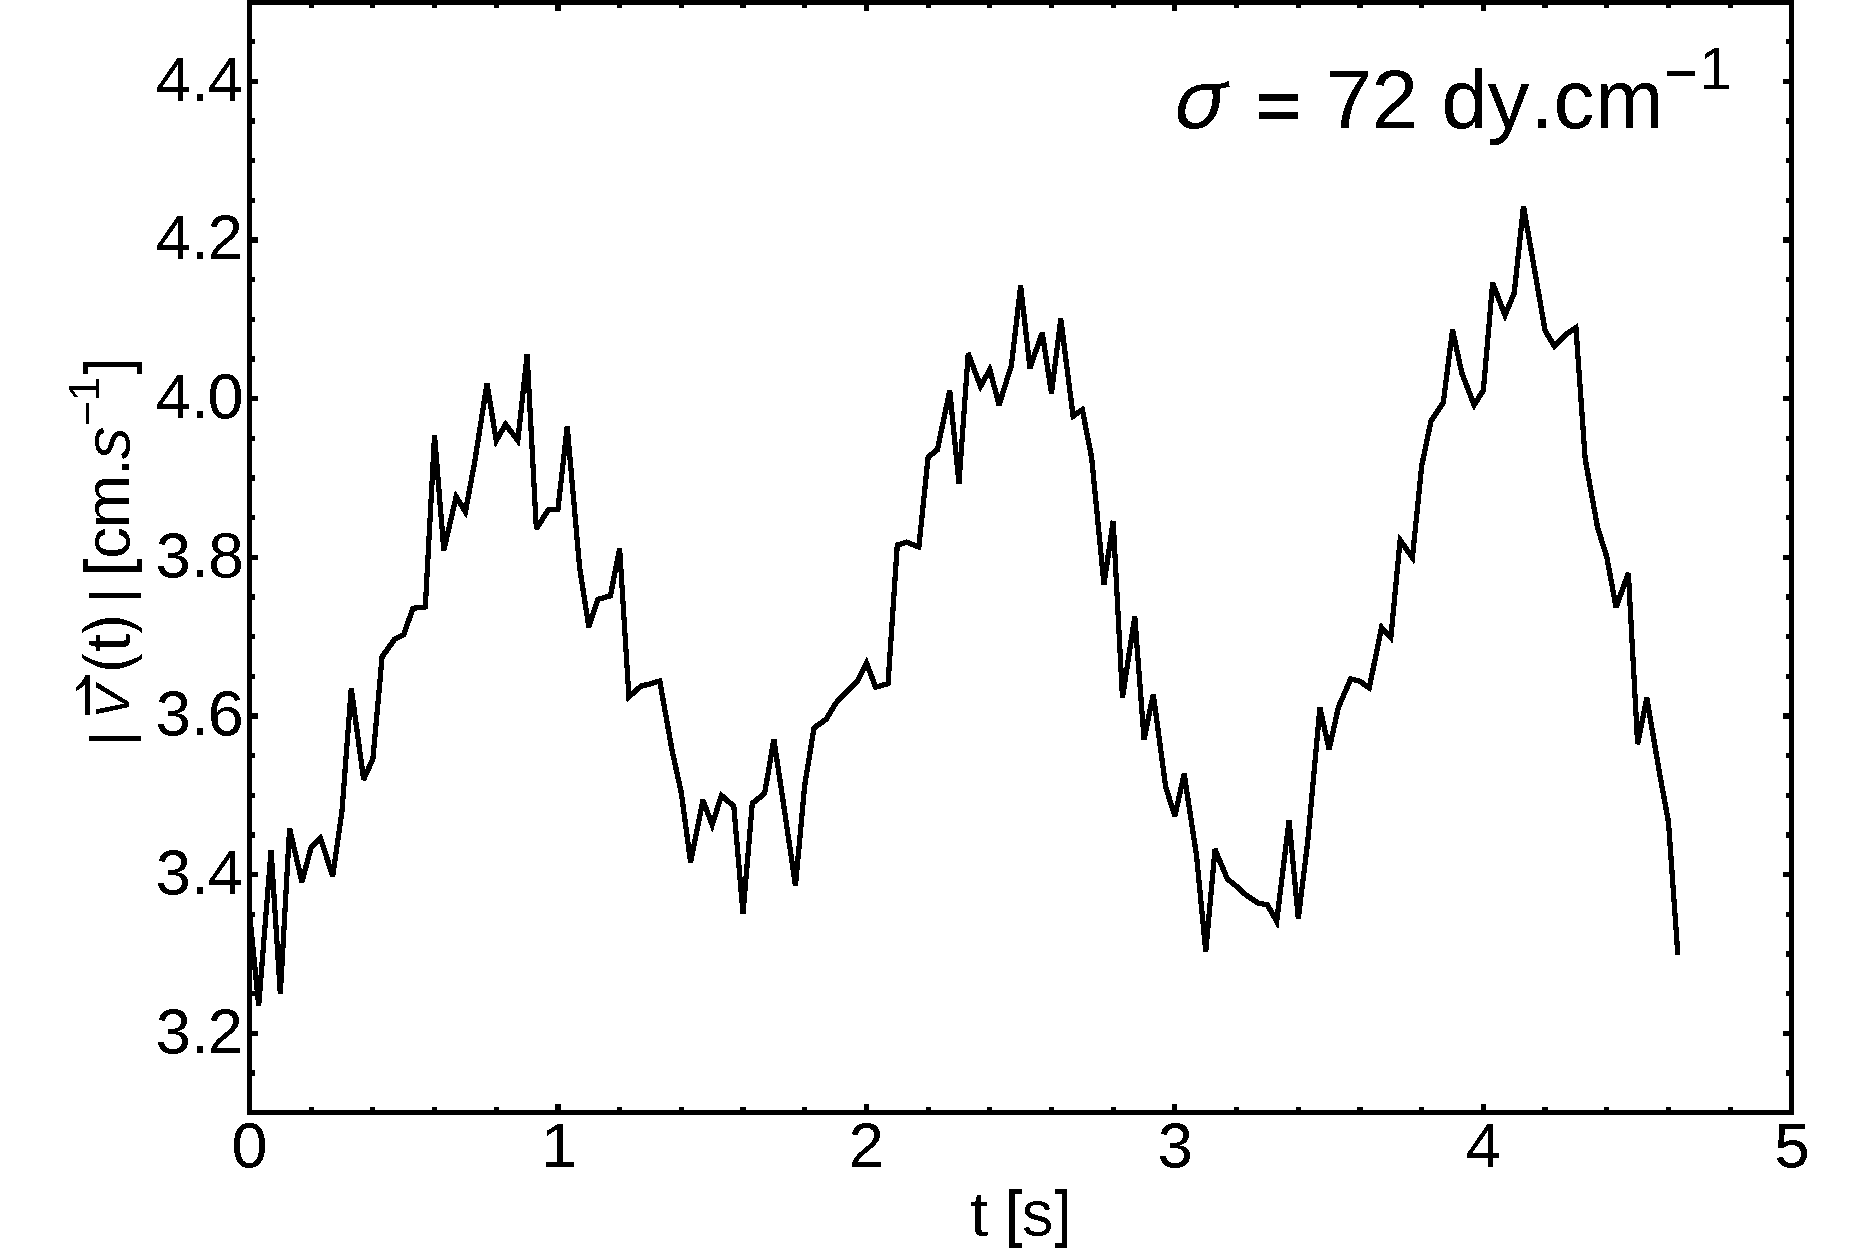
\includegraphics[width=\textwidth]{uvst_sigma_a.pdf}
		% \caption{$\xi > \xi_{c}$}\label{fig:uvst_sigma_a}		
	\end{minipage}
	\begin{minipage}[t]{0.3\linewidth}
		\centering
		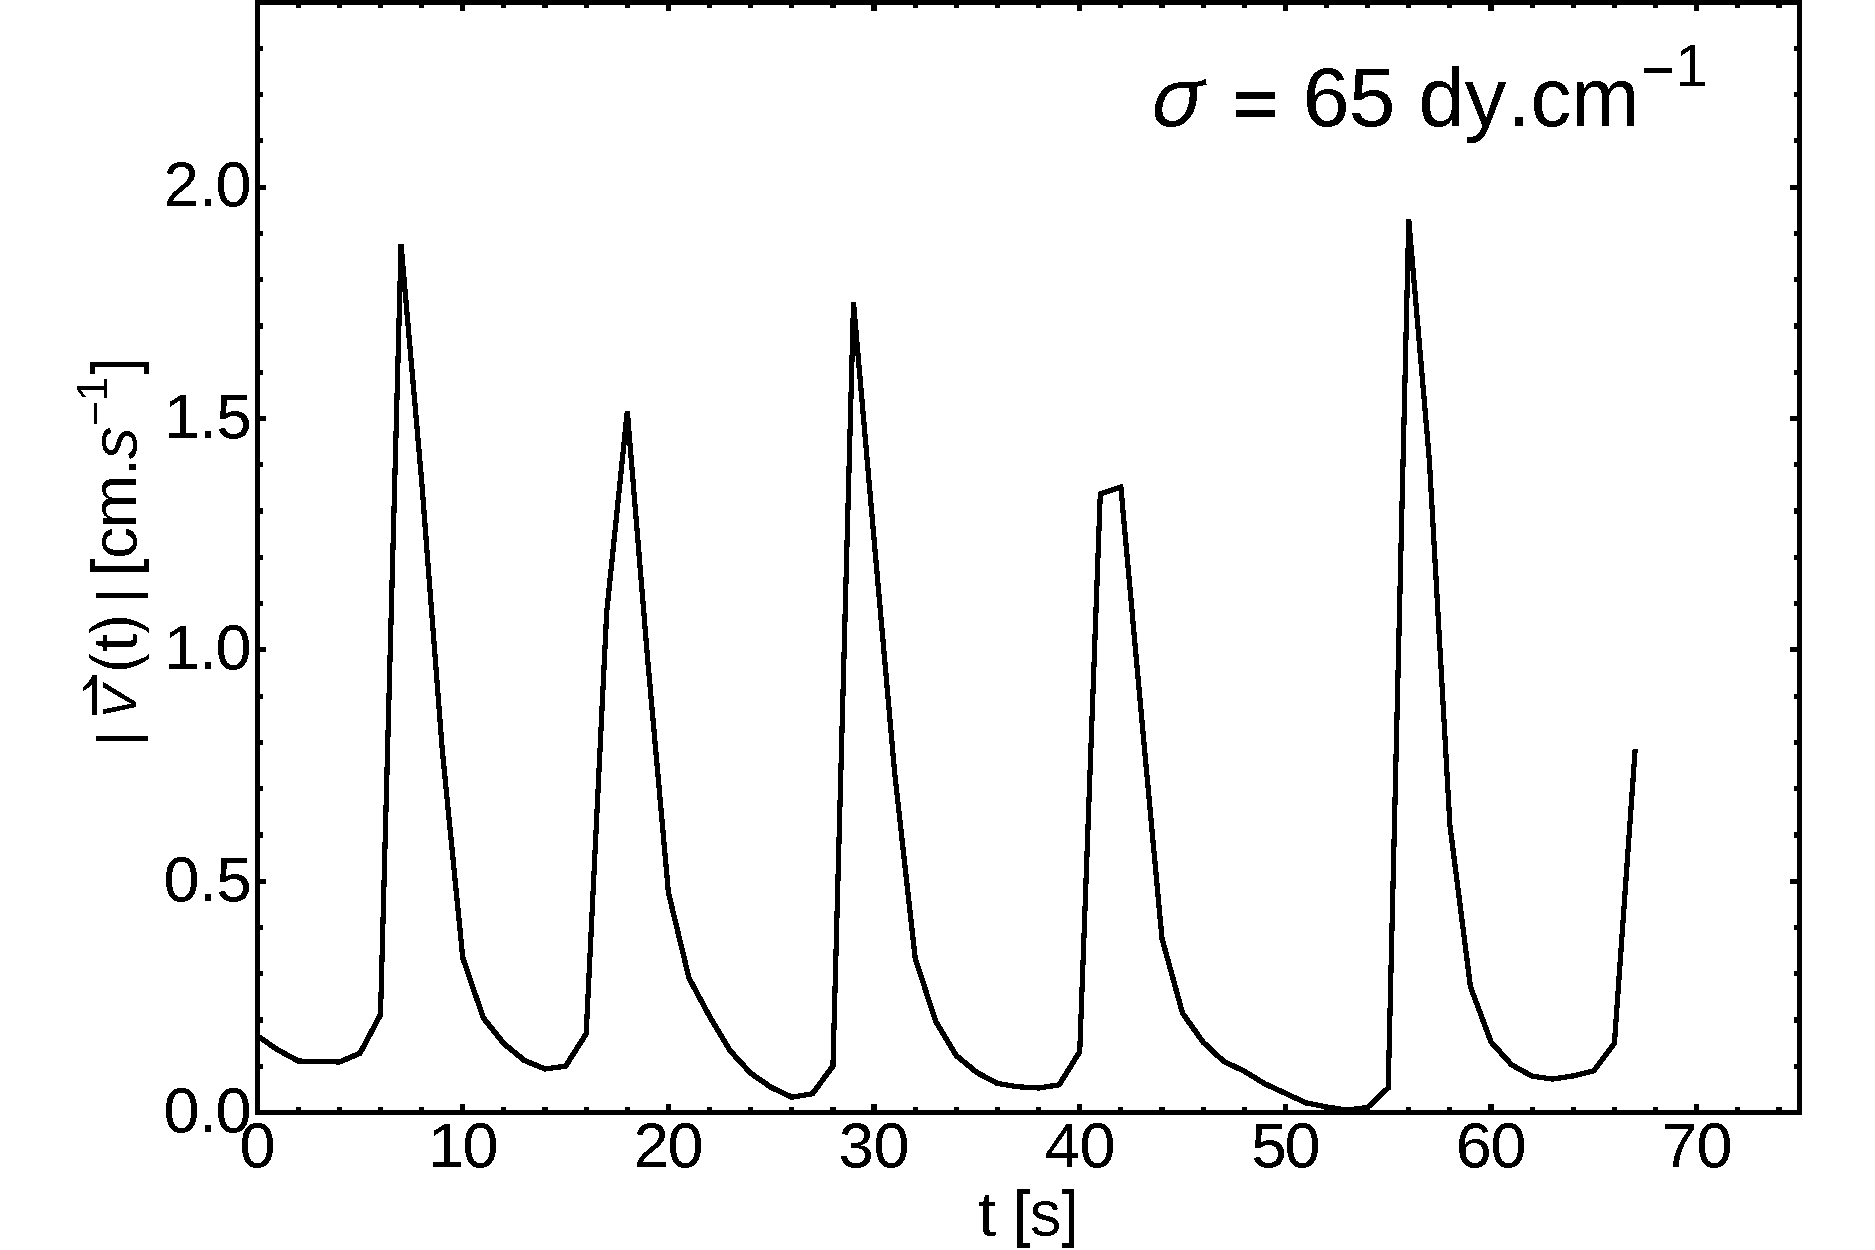
\includegraphics[width=\textwidth]{uvst_sigma_b.pdf}
		% \caption{$\xi \simeq \xi_{c}$}\label{fig:uvst_sigma_b}
	\end{minipage}
	\begin{minipage}[t]{0.3\linewidth}
		\centering
		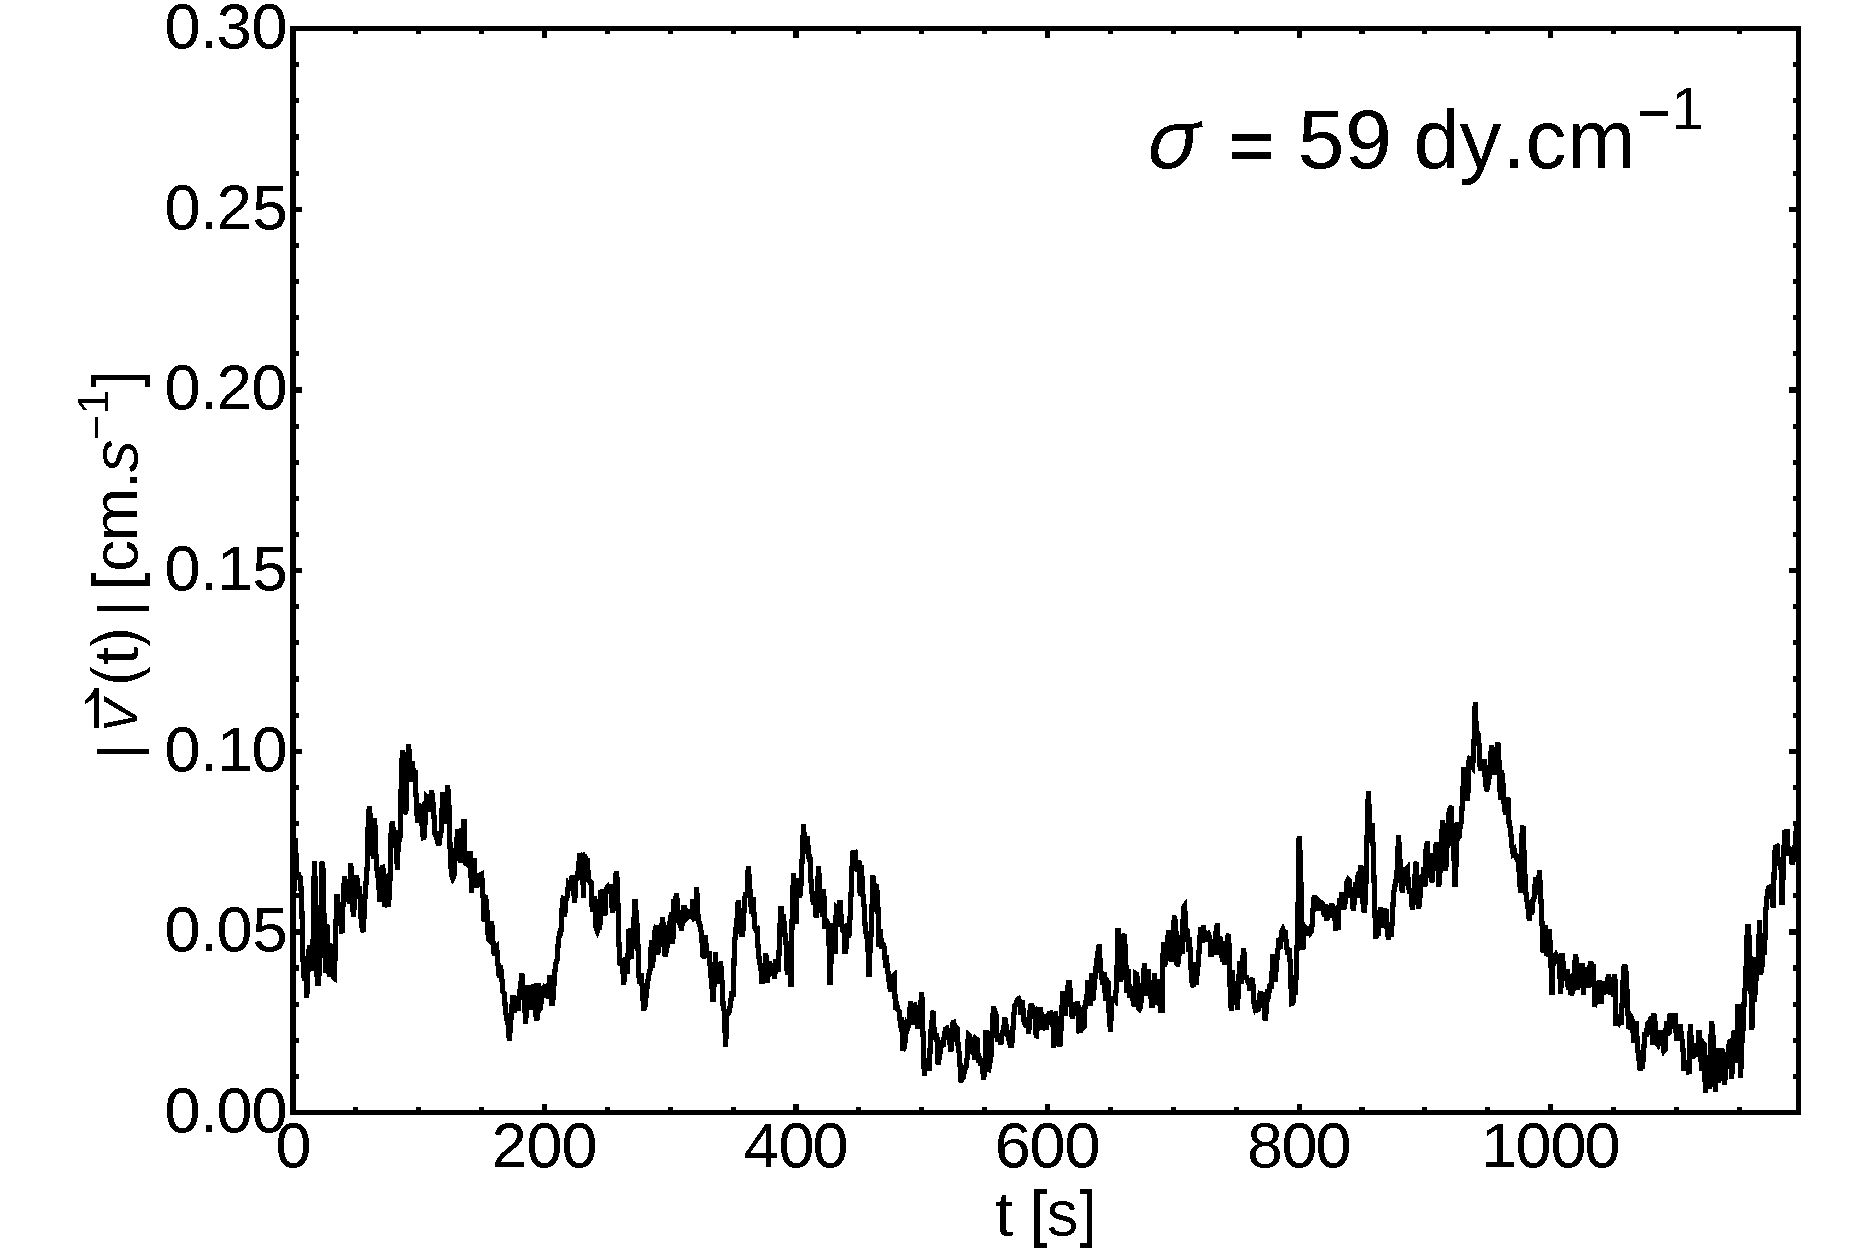
\includegraphics[width=\textwidth]{uvst_sigma_c.pdf}
		% \caption{$\xi < \xi_{c}$}\label{fig:uvst_sigma_c}
	\end{minipage}
	\caption{$\xi > \xi_{c}$, $\xi \simeq \xi_{c}$ and $\xi < \xi_{c}$}\label{fig:uvst_sigma}
\end{figure*}
\section{Summary}
\label{sec:summary}
We presented a simple system of self-propelling cboat at the air-water interface. A cboat, when placed at the air-water interface, is spontaneously set in motion by the interfacial tension gradients. The interfacial tension gradients are set up by the CA molecules which decrease the surface tension of water. The cboat speed continuously decreases with time due to the dissolution of CA in water. We fitted the cboat to an exponential decay in time to obtain the life time of the cboat $\tau \sim 35\ \mathrm{min}$. Furthermore, we observed oscillations in the cboat speed at shorter time scales than the life time of the cboat. These oscillations occur as a result of competition between the driving (interfacial tension) forces and damping (viscous drag) forces. We described the oscillations using a dimensionless parameter $\xi$ which quantifies the relative strengths of the driving and damping forces. We experimentally found a critical value, $\xi_{c} \simeq 5625$ at which the cboat moves with terminal velocity. We varied $\xi$ by changing the air-water interfacial tension using SDS. The oscillation frequency is governed by the advection time scale $\tau_{A} \sim \frac{R}{U_{M}}$, which is the time required for a CA molecule to be advected by the Marangoni flow to a distance $R$.

\begin{acknowledgement}
VSA, DKS, and MMB were supported by the Collective Interactions Unit at the Okinawa Institute of Science and Technology. MMB acknowledges L. Mahadevan for introducing the camphor boat system and subsequent scientific discussions, and D. Vu Anh for help with preliminary experiments. The authors acknowledge Kenneth J. Meacham III for help with experiments.
\end{acknowledgement}

% \begin{suppinfo}

% This will usually read something like: ``Experimental procedures and
% characterization data for all new compounds. The class will
% automatically add a sentence pointing to the information on-line:

% \end{suppinfo}

% The appropriate \bibliography command should be placed here.
% Notice that the class file automatically sets \bibliographystyle
% and also names the section correctly.

\bibliography{CBoat2-v2}

\end{document}
